\section{User Study: \papertitle\ prototype implemented on an Android Smartwatch}

To test the performance of \papertitle, we have implemented \papertitle\ 4 and \papertitle\ 5 on the Sony SmartWatch 3 running Android 4.4. We have also implemented Autodesk Research's Swipeboard on our system for comparison purpose since it performs well on smartwatches compared to other existing keyboards. Swipeboard's performance is compatible or better than that of Zoomboard \cite{swipeboard}. However, Swipeboard has a QWERTY based keyboard layout. In order to separate the factor of keyboard layout from character arrangement, we have also implemented a Swipeboard-like keyboard in alphabetical order. To make the keyboard consistent, we have removed the button with 4 characters: r, t, y, u and allowed buttons to have only 3 characters each. For all of the keyboards we have implemented, the users can delete characters (backspace) or enter a space (spacebar) in a consistent way. To delete a character, users can swipe left on the text entry space. To enter a space, the users can swipe right on the text entry space. Figure 7 shows all the keyboard designs.

\begin{figure*}
\begin{subfigure}{.24\textwidth}
  \centering
  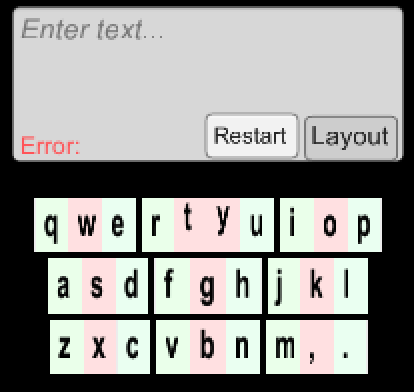
\includegraphics[width=.8\linewidth]{figures/F8-1.png}
  \caption{}
  \label{fig:f8a}
\end{subfigure}%
\begin{subfigure}{.24\textwidth}
  \centering
  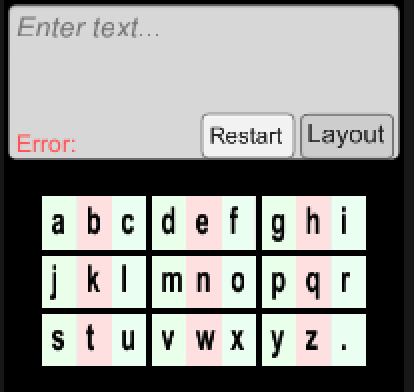
\includegraphics[width=.8\linewidth]{figures/F8-2.png}
  \caption{}
  \label{fig:f8b}
\end{subfigure}
\begin{subfigure}{.24\textwidth}
  \centering
  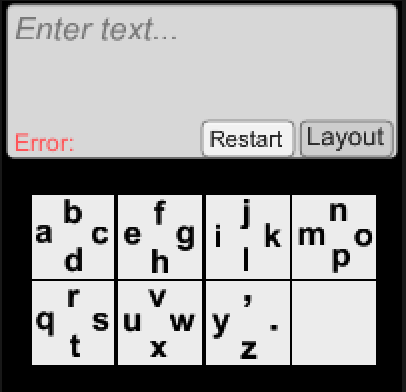
\includegraphics[width=.8\linewidth]{figures/F8-3.png}
  \caption{}
  \label{fig:f8c}
\end{subfigure}
\begin{subfigure}{.24\textwidth}
  \centering
  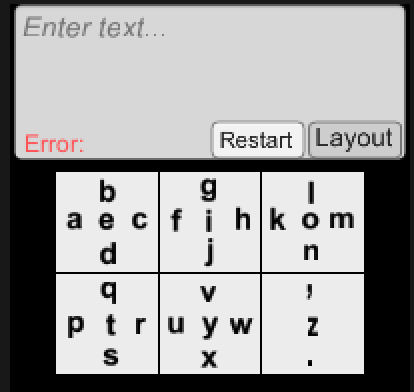
\includegraphics[width=.8\linewidth]{figures/F8-4.png}
  \caption{}
  \label{fig:f8d}
\end{subfigure}
\caption{Keyboard layout on smartwatch (a) Swipeboard (b) Swipeboard (Alphabetical) (c) \papertitle 4 (d) \papertitle 5}
\label{fig:f8}
\end{figure*}

\subsection{Participants}
We have recruited 12 participants for this test. Of these 12 participants, 7 were male and 5 were female. The average age is 24 years old. 9 participants stated that they could perform blind-typing on a PC keyboard. 10 participants were right-handed. All participants own touchscreen smartphones and 5 of them have used a smartwatch before.

\subsection{Task}
Participants were given a total of 2 minutes to get familiar with each type of keyboard before the test. They were told to use their index finger of their dominant hand to enter text. Each participant had to run 6 task blocks per keyboard, where the users were asked to type out 5 phrases per task block. In other words, they were asked to type out 30 phrases for each keyboard layout in a predetermined counter-balanced order. All in all, each user saw a total of 120 different phrases throughout the test. These test phrases were drawn randomly from the 500-phrase corpus compiled by MacKenzie and Soukoreff \cite{phrase-set}. A big screen in front of the user was used to display a phrase and the user then entered the displayed text on the smartwatch keyboard. The screen displayed the current phrase the user was supposed to be typing. The screen switched to showing the next phrase only when the participant finished typing out the current phrase. The reason for displaying each phrase on the screen rather than asking users to memorize each phrase was to avoid memorability bias. In all of the trials, we have instructed the participants to correct their mistakes as they were typing on the keyboard. They can swipe left on the text entry space to delete a character they have mistyped and then retype the correct character. However, if they fail to notice a mistake and only realize it after typing several more characters, they would then ignore the mistake and continue typing normally. At the end of the test, participants completed a short questionnaire and a short interview.

\subsection{Result and Discussion}

\subsubsection{Text Entry Speed}

\begin{figure}[t]
  \begin{subfigure}{1\columnwidth}
  \centering
  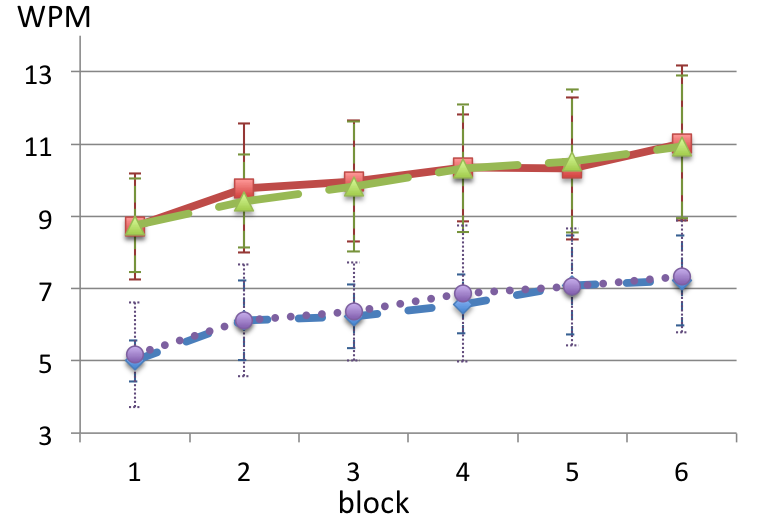
\includegraphics[width=.8\columnwidth]{figures/F9-1.png}
  \caption{}
  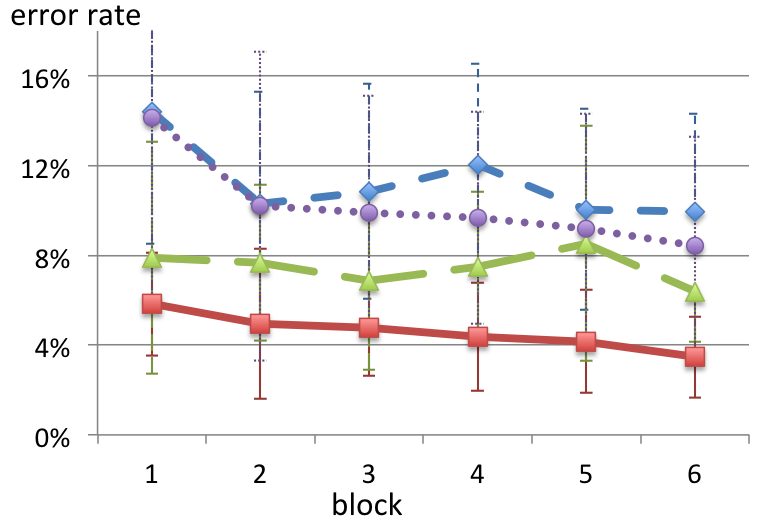
\includegraphics[width=.8\columnwidth]{figures/F9-2.png}
  \caption{}
  \label{fig:f9}
  \end{subfigure}
  \caption{ Quantitative results of user study for \papertitle verification (a) WPM (b) error rate}
\end{figure}

Figure 8 (a) shows the aggregated WPM results of the 12 users (including error correction time). Swipeboard (QWERTY layout) had 5.0 WPM in the first block. After more than half an hour of training, the typing speed rose to 7.3 WPM in the last block. The WPM curve of Swipeboard (QWERTY) is slightly lower and almost overlaps with that of Swipeboard (alphabetical), with a 5.3 WPM in the first block and 7.4 WPM in the end. The result suggests that the QWERTY keyboard layout does not help the users type faster than users who use an alphabetical keyboard layout. It also supports our design decision of using alphabetical grouping. Two of our users mentioned that the feeling of typing on Swipeboard (QWERTY) is totally different from typing on a mechanical keyboard, despite the fact that both users are capable of blind-typing. It is hard for them to transfer their muscle memory of using a mechanical QWERTY layout to the Swipeboard input method even if it is based on QWERTY. This might be a possible reason why QWERTY is not particularly helpful for character location memorization.

The WPM of \papertitle\ 4 and \papertitle\ 5 are 8.7 and 8.8 respectively in the first block, and 11 and 10.9 respectively in the last block. \papertitle\ 4 and \papertitle\ 5 are comparable in terms of speed even after the users got some practice. The WPM of \papertitle\ group is much higher than that of the Swipeboard group. There is a significant performance difference among all the test data (F(1,262)=283.4, p << .001). The initial speed of the \papertitle\ group is even faster than that of the trained Swipeboard group. It shows that the speed gap between \papertitle\ and Swipeboard is at about 4 WPM across all tests. This might imply a non-converging typing speed between these 2 groups even after long-term training. The superiority of \papertitle\ in speed is due to the second design requirement. \papertitle\ is expected to have a shorter reaction time for each character. It takes 1 swipe for each character while Swipeboard requires 2.

\subsubsection{Error Rate}
In Figure 8 (b), the error rate in the beginning is comparable between Swipeboard (QWERTY) and Swipeboard (alphabetical). Though, after a short training session, Swipeboard (alphabetical) shows a slightly lower error rate in the last 3 blocks (F(1,64) = 2.17, p = 0.14). Six users reported that they made more mistakes when they tried to type out the 't' and 'y' characters located on the 'rtyu' button of the Swipeboard (QWERTY). One user found the 'rtyu' button inconsistent and confusing because that button consisted of 4 characters while the other 8 buttons in the layout consisted of only 3. 

The average error rate for the Swipeboard group (10.9\%) is about half of the error rate for the \papertitle\ group (5.8\%) across all tests (F(1,262)=71.9, p << .001). This could be explained by 2 factors. Firstly, Swipeboard users needed to make 2 swipes in order to type a single character, which increased the error rate due to the extra swipe. \papertitle\ users needed to make only 1 swipe per character. Secondly, the inconsistent swipe directions in the first (8 directional swipes + 1 tap) and the second layer (2 directional swipes + 1 tap or 4 directional swipes) introduce a higher error rate. Users also reported that \papertitle\ is more intuitive to use.

For in-group comparison of \papertitle, \papertitle\ 4 had a significantly lower error rate (4.4\% on average, 3.4\% for the last block) compared to \papertitle\ 5 (7.4\% on average, 6.3\% for the last block) (F(1,130)=26.4, p < .001). We already noticed this phenomenon in our previous user study when designing \papertitle, and we believe that it is caused by inconsistent design and combination of 2 different types of movement: tap and swipe. Some participants mentioned that their tap was accepted as a swipe and that they could not distinguish which is more likely to happen. 

\subsubsection{User Survey}

\begin{figure}[h]
  \begin{subfigure}{1\columnwidth}
  \centering
  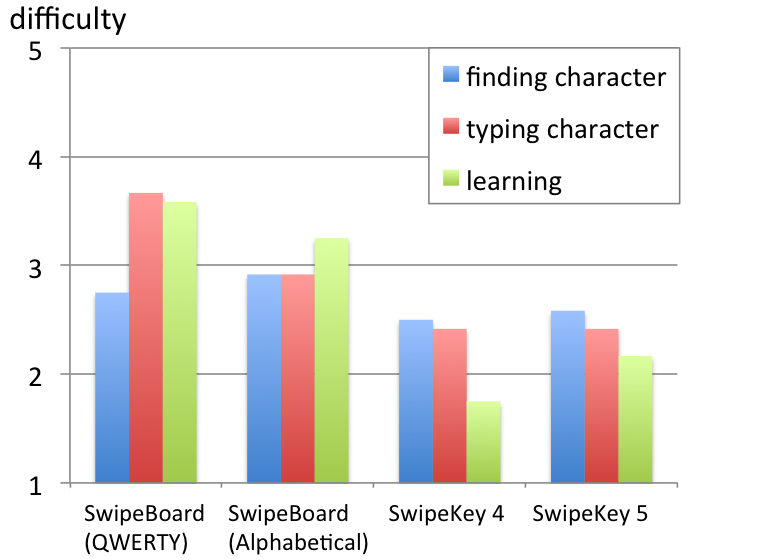
\includegraphics[width=.8\columnwidth]{figures/F10-1.png}
  \caption{}
  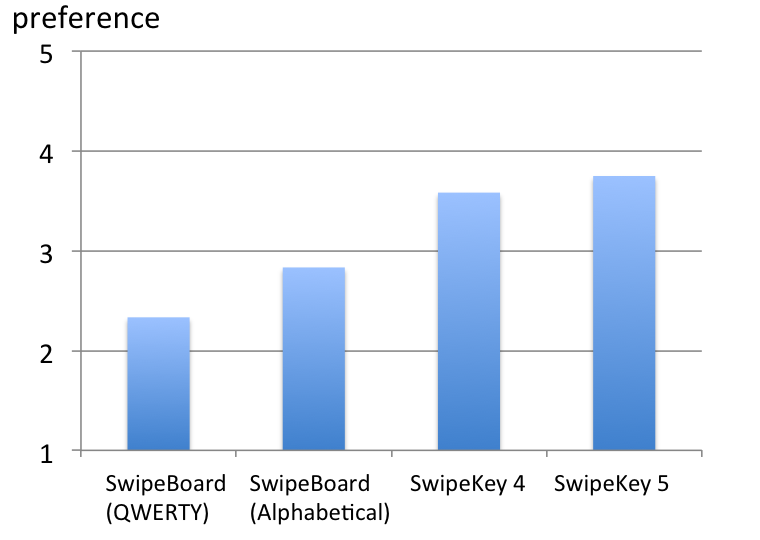
\includegraphics[width=.8\columnwidth]{figures/F10-2.png}
  \caption{}
  \label{fig:f10}
  \end{subfigure}
  \caption{ (a) User rating of difficulty on a 5-point Likert scale for finding a character, typing a located character, and learning how to use different keyboards. (b) User preference of different keyboards}
\end{figure}

We summarize 3 different kinds of difficulty rating of keyboard layouts in Figure 9 (a). There is no significant difference in finding a character between Swipeboard (QWERTY) and Swipeboard (alphabetical). However, there are 3 users who said that they found it more difficult to find characters on the alphabetically ordered keyboard. Their difficulty rating for finding characters on the alphabetically ordered keyboard is much higher than that of other users (average 3.9 point of the 3 users compared with 2.7 point of 12 users). The rest of the users did not find the QWERTY layout more helpful.

Typing characters on Swipeboard (QWERTY) is the most difficult. This is revealed in our interview with users. Our users mentioned that “It is hard to swipe 'r' and 't', and it continuously enters the wrong character“, “Sometimes, my swipe on the first layer keeps entering the wrong group of characters”, or “The 't' and 'y' are hard to type”. 
Considering the difficulty of learning for each keyboard, we see that \papertitle\ is easier to learn compared to Swipeboard (F(1,42)=21.1,  p=0.004). One of the participants said that it took him a while to get accustomed to Swipeboard, but he could use \papertitle\ immediately. However, those who had difficulty in finding characters do feel that there is a high learning curve for \papertitle (average 3.5 compared with total average 2.0).

In Figure 9 (b), the preference for \papertitle\ in a 5-point Likert scale is higher than that of Swipeboard (F(1,42)=17.8,  p=0.013). Most of the users said that they prefer SwipeKey because it is intuitive and easier to use compared to Swipeboard. However, there is still one participant that prefers Swipeboard (QWERTY) due to the QWERTY layout, despite the fact that both speed and error rate of that particular participant are better with \papertitle.
